\section*{Materials and methods}

\subsection*{Data}

Two different previously-published datasets were used here:

\begin{enumerate}

\item Diffusion MRI data from a previous study of properties of the white matter
across the lifespan\cite{yeatman2014lifespan}, containing dMRI data from 76
subjects with ages 6-50. These data were measured in a GE Discovery 750 3T MRI
scanner at the Stanford Center for Cognitive and Neurobiological Imaging. The
Stanford University IRB approved the procedures of this study. Informed consent
was obtained from each adult participant, and assent for participation was
provided by parents/guardians for children. Voxel resolution was
\num{2x2x2}$mm^3$ with 96 non-colinear directions measured with a $b=2000$
$\frac{sec}{mm^2}$ and 30 non-colinear directions measured with a $b=1000$
$\frac{sec}{mm^2}$. Data was preprocessed to correct for subject motion and the
diffusion tensor model \cite{basser1994mr} was fit in every voxel, using a
robust fit \cite{chang2005restore}. These data were acquired using a dual spin
echo sequence, in which there is sufficient time for eddy currents to subside
between the application of the gradients and the image acquisition, so no eddy
current correction was appliced. We will refer to this dataset as WH.

\item Diffusion MRI from from a previous study of the corticospinal tract
profile in patients with amyotrophic lateral sclerosis
(ALS)\cite{sarica2017corticospinal}, containing data from 24 ALS patients and 24
demographically matched healthy controls. These data were measured in a GE
Discovery 750 3T MRI scanner at the Institute of Bioimaging and Molecular
Physiology in Catanzaro. Informed consent was provided as approved by the
Ethical Committee of the University ``Magna Graecia'' of Catanzaro. Voxel
resolution was \num{2x2x2} $mm^3$ and 27 non-colinear directions were
measured with a $b=1000$ $\frac{sec}{mm^2}$. Here, both motion correction and
eddy current correction were applied before modeling the diffusioon tensor in
each voxel. We will refer to this dataset as ALS.

\end{enumerate}

Data from both of these studies was processed in a similar manner, using the
Matlab Automated Fiber Quantification toolbox (AFQ) \cite{yeatman2012tract}:
streamlines representing fascicles of white matter tracts were generated
using a determinstic tractography algorithm that follows the prinicpal diffusion
direction of the diffusion tensor in each voxel (STT \cite{basser2000vivo}).
Major tracts were identified using multiple criteria: streamlines are selected
as candidates for inclusion in a bundle of streamlines that represents a tract
if they pass through known inclusion ROIs and do not pass through exclusion ROIs
\cite{wakana2007reproducibility}. In addition, a probabilistic atlas is used to
exclude streamlines which are unlikely to be part of a tract \cite{Hua2008-sh}.
Each streamline is resampled to 100 nodes and the robust mean at each location
is calculated by estimating the 3D covariance of the location of each node and
excluding streamlines that are more than 5 standard deviations from the mean
location in any node. Finally, a tract profile of tissue properties in each
tract was created by interpolating the value of MRI maps of these tissue
properties to the location of the nodes of the resampled streamlines designated
to each tract. In each of 100 nodes, the values are summed across streamlines,
weighting the contribution of each streamline by the inverse of the mahalnobis
distance of the node from the average  of that node across streamlines. This
means that streamlines that are more representative of the tract contribute more
to the tract profile, relative to streamlines that are on the edge of the tract.

This process creates tract profiles, in which diffusion measures are quantified
and averaged along twenty major fiber tracts. Here, we use only the mean
diffusivity (MD) and the fractional anisotropy (FA) of the diffusion tensor, but
additional dMRI-based maps or maps based on other quantitative MRI measurements
can also be used. These tract profiles, along with the phenotypical data we wish
to explain or predict, form the input to the SGL algorithm. In a domain-agnostic
machine learning context, the phenotypical data comprise the target variables
while the tract profiles form the feature or predictor variables (See
Fig~\ref{fig:group-structure}).

\subsection*{Sparse Group Lasso}

Before fitting a model to the data, imputation and standardization are
performed. Missing node values (e.g., in cases where AFQ designates a node as
not-a-number) are imputed via linear interpolation. Care is taken not to
interpolate across the boundaries between different tracts. Some diffusion
metrics will have naturally larger variance than others and may therefore
dominate the objective function and make the SGL estimator unable to learn from
the lower variance metrics. For example, fractional anisotropy (FA) is bounded
between zero and one and could be overwhelmed by an unscaled higher-variance
metric like the mean diffusivity (MD). To prevent this we remove each feature's
mean and scale it to unit variance (z-score) using the
\lstinline{StandardScaler} from scikit-learn \cite{scikit-learn}. Scaling is
performed separately within each cross-validation set's training or testing data
to prevent leakage of information between the testing and training
sets\cite{kaufman2012leakage}.

After scaling and imputation, the tractometry data and target
phenotypical data can be organized in a linear model:
\begin{equation}
    y = \mathbf{X} \beta + \epsilon,
    \label{eq:lm}
\end{equation}
where $y$ is the phenotype -- categorical, such as a clinical diagnosis,
or continuous numerical, such as the subject's age. The tractometry
data is represented in the feature matrix $\mathbf{X}$, with rows
corresponding to different subjects, and columns corresponding
to diffusion measures at different nodes within each tract. The
relationship between tractometric features and the phenotypic target is
characterized by the coefficients in $\beta$. The error term, $\epsilon$
is an unobserved random variable that captures the error in the model.
We denote our prediction of the targer phenotype as $\hat{y}$ and the
coefficients that produce this prediction as $\hat{\beta}$, so that
\begin{equation}
    \hat{y} = \mathbf{X} \hat{\beta},
    \label{eq:lm-approx}
\end{equation}
without the error term, $\epsilon$. In general, the feature matrix
$\mathbf{X}$ has dimensions $S \times (T \times N \times M)$, where $S$
is the number of subjects, $T$ is the number of white matter tracts,
$N$ is the number of nodes in each tract, and $M$ is the number of
diffusion metrics calculated at each node. Typically, $T = 20$, $N =
100$, and $2 \le M \le 8$, resulting in $\sim 4,000 - 16,000$ features.
Conversely, many dMRI studies have between a few dozen and a few
hundred subjects, yielding a feature matrix that is wide and short.
Even in cases where more than a thousand subjects are measured (e.g.,
in the Human Connectome Project, where 1,200 subjects were measured
\cite{VanEssen2012}), the problem is ill-posed: the high dimensionality
of this data requires regularization to avoid overfitting and generate
interpretable results.

Here, we propose that in addition to regularizing the coefficients
in $\hat{\beta}$, we can also capitalize on our knowledge of the
group structure of the tract profile features in $\mathbf{X}$. The
tract-metric combinations form a natural grouping. For example, we
expect that MD features within the left arcuate fasciculus will
co-vary across individuals. Likewise for FA values within the right
corticospinal tract (CST) and so on. This group structure is represented
in Fig~\ref{fig:group-structure}, which depicts the linear model
$\hat{y} = \mathbf{X} \hat{\beta}$. Thus, we seek a regularization
approach that will fit a linear model with anatomically-grouped
covariates, where we expect to observe both groupwise sparsity, where
the number of groups (tract/metric combinations) with at least one
non-zero coefficients is small, as well as within-group sparsity, where
the number of non-zero coefficients within each non-zero group is small.
The sparse group lasso (SGL) is a penalized regression technique that
satisfies exactly these criteria\cite{simon2013sparse}. It solves for a
coefficient vector
$\hat{\beta}$ that satisfies
\begin{equation}
    \hat{\beta} = \min_\beta \frac{1}{2}
    ||y - \displaystyle \sum_{\ell = 1}^{G}
    \mathbf{X}^{(\ell)} \beta^{(\ell)}||_2^2
    + \lambda_1 \displaystyle \sum_{\ell = 1}^{G}
    \sqrt{p_\ell} ||\beta^{(\ell)}||_2
    + \lambda_2 ||\beta||_1,
    \label{eq:sgl}
\end{equation}
where $G$ is the number of groups $\mathbf{X}^{(\ell)}$ is the submatrix
of $\mathbf{X}$ corresponding to group $\ell$, $\beta^{(\ell)}$ is
the coefficient vector for group $\ell$ and $p_\ell$ is the length of
$\beta^{(\ell)}$. In the tractomtetry setting, $G = T \times M$ and
$\forall \ell: p_\ell = 100$. The first term is the mean square error
loss, $L_{\text{mse}}$, as in the standard linear regression framework.
The second and third terms encourage groupwise sparsity and overall
sparsity, respectively. If $\lambda_1 = 0$ and $\lambda_2 = 1$, the
SGL reduces to the traditional lasso\cite{tibshirani1996regression}.
Conversely, if $\lambda_1 = 1$ and $\lambda_2 = 0$, the SGL reduces to
the group lasso\cite{yuan2006model}.

\begin{figure}[!h]
    \centering
    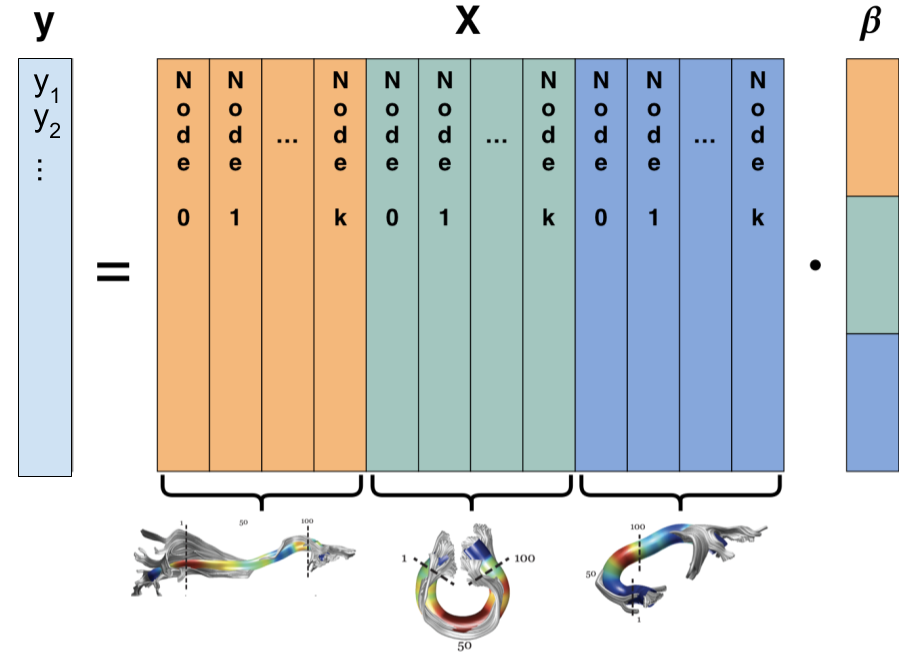
\includegraphics[width=0.65\textwidth]{dMRI_group_structure.png}
    \caption{{\bf dMRI group structure.}
        The phenotypical target data and tractometric features can
        be organized into a linear model, $\hat{y} = \mathbf{X}
        \hat{\beta}$. The feature matrix $\mathbf{X}$ is color-coded
        to reveal a natural group structure: the left (orange) group
        contains $k$ features from the inferior fronto-occipital
        fascicle (IFOF), the middle (green) group contains $k$ features
        from the corpus callosum, and the right (blue) group
        contains $k$ features from the uncinate. The coefficients in
        $\hat{\beta}$ follow the same natural grouping. Fascicle image
        reproduced with permission from Ref~\cite{yeatman2012tract}
        Figure 1.
    }
    \label{fig:group-structure}
\end{figure}


\subsubsection*{Incorporating transformations on $y$}

Often, the target variable $y$ is not in the domain in which the linear
model can be best fit to it. Equation \ref{eq:lm-approx} can be slightly
modified as:
\begin{equation}
    \hat{y} = f^-1(\mathbf{X} \hat{\beta}),
    \label{eq:lm-transform}
\end{equation}
where the transformation function $f^{-1}$ characterizes the transform
applied to the data before fitting the linear coefficients. For example,
an often-used transform is the logarithmic transform:
\begin{equation}
    f(\hat{y}) = \log_n(\hat{y})
    \label{eq:log-nonlinearity}
\end{equation}
In this case, the model is parametrized by one additional fit parameter,
$n$.

\subsubsection*{Classification of categorical $y$}
When the phenotypical target variable is categorical, as in the case of
explaining or predicting the presence of a clinical diagnosis, the SGL is
readily adapted to logistic regression, where the probability of a target
variable belonging to an arbitrary defined ``true'' class is the logistic
function of the result of the linear model,
\begin{equation}
    p(\hat{y} = 1) = \frac{1}{1 + \exp(\mathbf{X} \hat{\beta})},
    \label{eq:logit}
\end{equation}
or equivalently, the mean squared error loss function in Eq~\eqref{eq:sgl} is
replaced with the cross-entropy loss, which for binary classification is the
negative log likelihood of the SGL classifier giving the ``true'' label:
\begin{equation}
    L_{\text{mse}} \rightarrow L_{\log} =
    -\left(y \log(p) + (1 - y) \log(1 - p)\right).
    \label{eq:logloss}
\end{equation}

\subsection*{Implementation, cross-validation and metaparameter optimization}

For given values of $\lambda_1$ and $\lambda_2$, the cost function in equation
\ref{eq:sgl} can be optimized using proximal gradient descent methods
\cite{parikh2014proximal} here implemented as a custom proximal operator that is
then optimized using the C-OPT library\cite{copt}. This supplies an estimate of
the optimal $\hat{\beta}$ given a particular set of values for the
meta-parameters $\lambda_1$ and $\lambda_2$.

To objectively evaluate the model and guard against over-fitting, we used a
nested cross-validation scheme, depicted in Fig~\ref{fig:cross-val} for the
categorical classification case. The input data is shuffled and then decomposed
into $k$ batches, hereafter referred to as folds. For the ALS dataset we used
$k=10$ and for the WH dataset $k=5$. For each unique fold, we hold that fold out
as the test\textsubscript{outer} set and let the remaining data comprise the
train\textsubscript{outer} set, with the subscript indicating the depth of the
nested decomposition. We further decompose each train\textsubscript{outer} set
into three folds, and again for each unique fold, we hold out that fold as the
test\textsubscript{inner} set and let the remaining data comprise the
train\textsubscript{inner} set. At level-1 of the decomposition, we fit an SGL
model using fixed regularization meta-parameters $\lambda_1$ and $\lambda_2$,
training the model using train\textsubscript{inner} and evaluating the fit on
test\textsubscript{inner}. We find the optimal values for $\lambda_1$ and
$\lambda_2$ using hyperoptimization, implemented using the hyperopt
library's \verb|fmin| function\cite{Bergstra_2015} with a tree of Parzen
estimators search algorithm\cite{bergstra2011algorithms}. For continuous
numerical $y$, \verb|fmin| searches for meta-parameter values that minimize the
median absolute error. This can also be done minimizing the root of the mean
squared error (RMSE) or to maximizing the coefficient of determination ($R^2$).
For binary categorical $y$ \verb|fmin| seeks to maximize the classification
accuracy. This can also be done maximizing the area under the receiver operating
curve (ROC AUC) or the average precision. Using hyperoptimization, we find
optimal regularization parameters and $\hat{\beta}$ for each
train\textsubscript{outer} set and then use those to predict values for data in
test\textsubscript{outer}. Thus each subject in the dataset has a predicted
phenotype derived from a model that never saw its particular subject's data.

The above procedure describes $k$-fold cross validation. In fact, we use
repeated $k$-fold cross validation on the outer level of the decomposition, so
that the input data is decomposed into $k$ folds, three times. Thus, each
subject has three predicted phenotypes. We then take the mean predicted value to
summarize the performance of the model. In the classification case, the
shuffling into folds is stratified such that each fold has a population that
preserves the percentage of each class found in the larger input data.

\begin{figure}[!h]
    \centering
    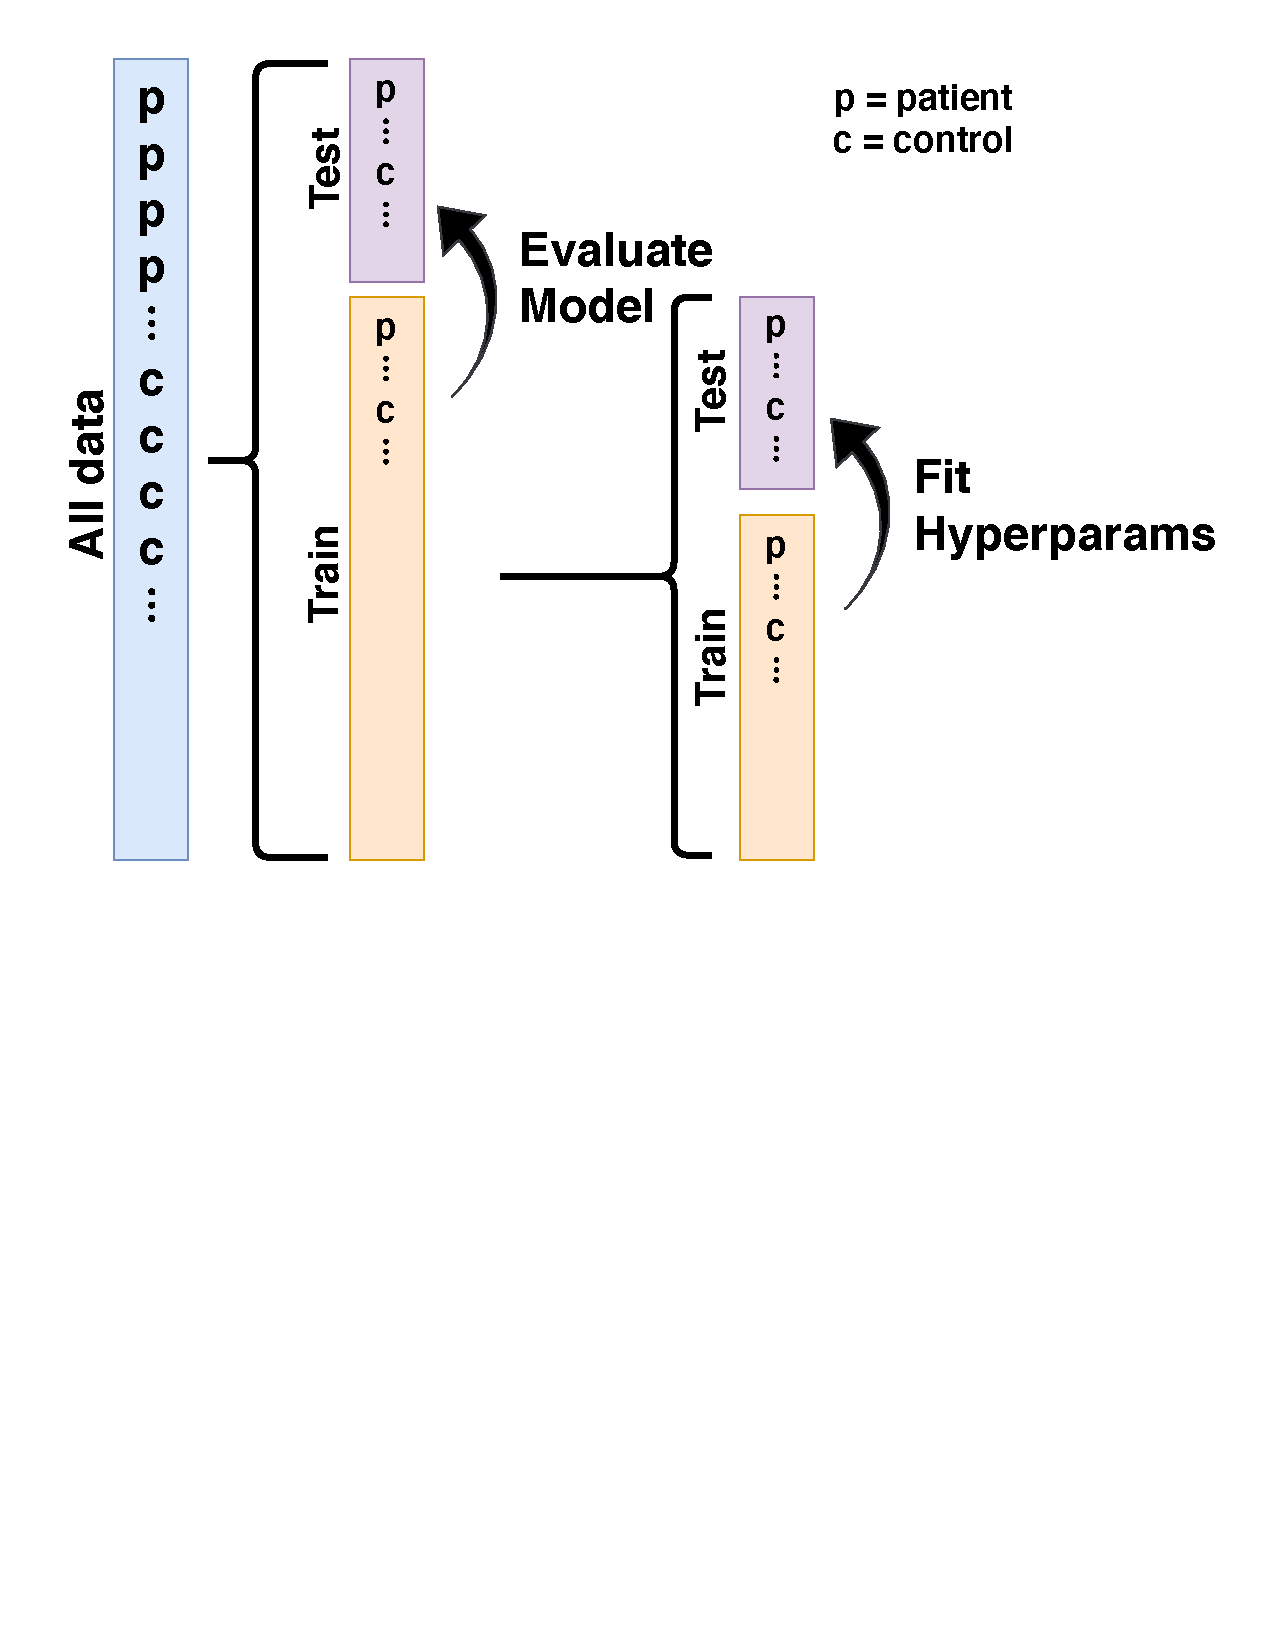
\includegraphics[width=0.55\textwidth]{nested-cross-validation.pdf}
    \caption{{\bf Nested $k$-fold cross-validation scheme.}
        We evaluate model quality using a nested $k$-fold cross
        validation scheme. At level-0, the input data is decomposed
        three times into $k$ shuffled groups and optimal hyperparameters
        are found for the level-0 training set. Optimization of these
        hyperparameters requires the use of the hyperopt library and
        many repeated evaluations of an SGL model over a search space
        of possible regularization parameters. These evaluations take
        place at level-1 of the decomposition, where the level-0 training
        set is further decomposed into three shuffled groups.
        For the ALS data, $k=10$. For the WH data, $k=5$.
    }
    \label{fig:cross-val}
\end{figure}

\subsection*{Software implementation}

The full software implementation of the SGL approach presented here is available
in a Python software package called AFQ-Insight, which is developed publicly in
\url{https://github.com/richford/afq-insight}. The version of the code used to
produce the results herein is also available in \ariel{Need to add Zenodo DOI}.
AFQ-Insight reads the target and feature data that has been processed by AFQ
from comma separated value (CSV) files conforming to the AFQ-Browser data
format\cite{yeatman2018browser} and represents them internally as
\lstinline{DataFrame} objects from the pandas Python
library\cite{mckinney2010data}. The software provides different options for
imputing missing data in the feature matrix. Missing interior nodes are imputed
using linear interpolation. For missing exterior nodes, the user may choose
between linear extrapolation and constant forward(back)-fill. Imputation uses
only values from adjacent nodes in the same white matter tract in the same
subject so there is no danger of data leakage from other subjects. It uses the
scikit-learn\cite{scikit-learn} library to decompose input data into separate
test and train datasets, to scale each feature to have zero mean and
unit variance, and to evaluate each fit in the hyperparameter search using
appropriate classification and regression metrics such as accuracy, area
under the receiver operating curve (AUC ROC), and coefficient of determination
($R^2$). For each set of hyperparameters, we solve the SGL using a custom
proximal operator supplied to the C-OPT library\cite{copt}. Appropriate
hyperparameters are found using the hyperopt library\cite{Bergstra_2015}.
